% Chapter 1

\chapter{Introducción General} % Main chapter title

\label{Chapter1} % For referencing the chapter elsewhere, use \ref{Chapter1} 
\label{IntroGeneral}

%----------------------------------------------------------------------------------------

% Define some commands to keep the formatting separated from the content 
\newcommand{\keyword}[1]{\textbf{#1}}
\newcommand{\tabhead}[1]{\textbf{#1}}
\newcommand{\code}[1]{\texttt{#1}}
\newcommand{\file}[1]{\texttt{\bfseries#1}}
\newcommand{\option}[1]{\texttt{\itshape#1}}
\newcommand{\grados}{$^{\circ}$}

%----------------------------------------------------------------------------------------
La idea de esta sección es presentar el tema de modo que cualquier persona que no conoce el tema pueda entender de qué se trata y por qué es importante realizar este trabajo y cuál es su impacto.

\section{Motivación}

\begin{figure}[h]
	\centering
	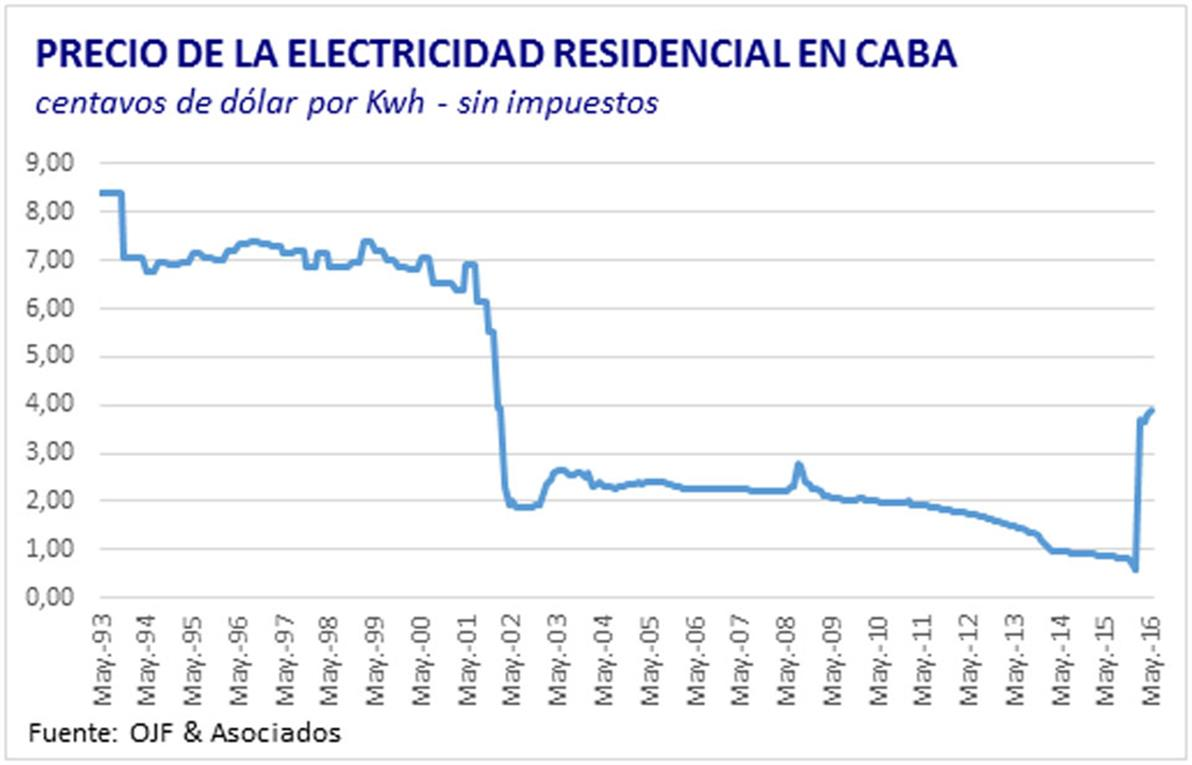
\includegraphics[width=12cm]{./Figures/1_1_costo_electricidad_caba.png}
	\caption{Evolución del costo de la energía eléctrica en la Ciudad Autónoma de Buenos Aires.}
	\label{fig:costo_caba}
\end{figure}

\section{Soluciones comerciales existentes}

\begin{figure}[h]
	\centering
	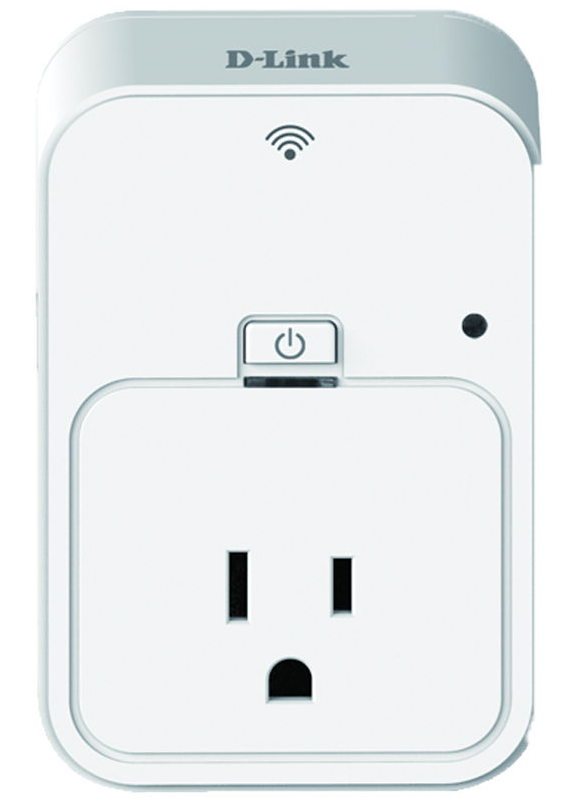
\includegraphics[width=6cm]{./Figures/1_2_DSP-W215.png}
	\caption{Smart Plug DSP-W215 de la empresa D-LINK}
	\label{fig:smartplug_dlink}
\end{figure}

\begin{figure}[h]
	\centering
	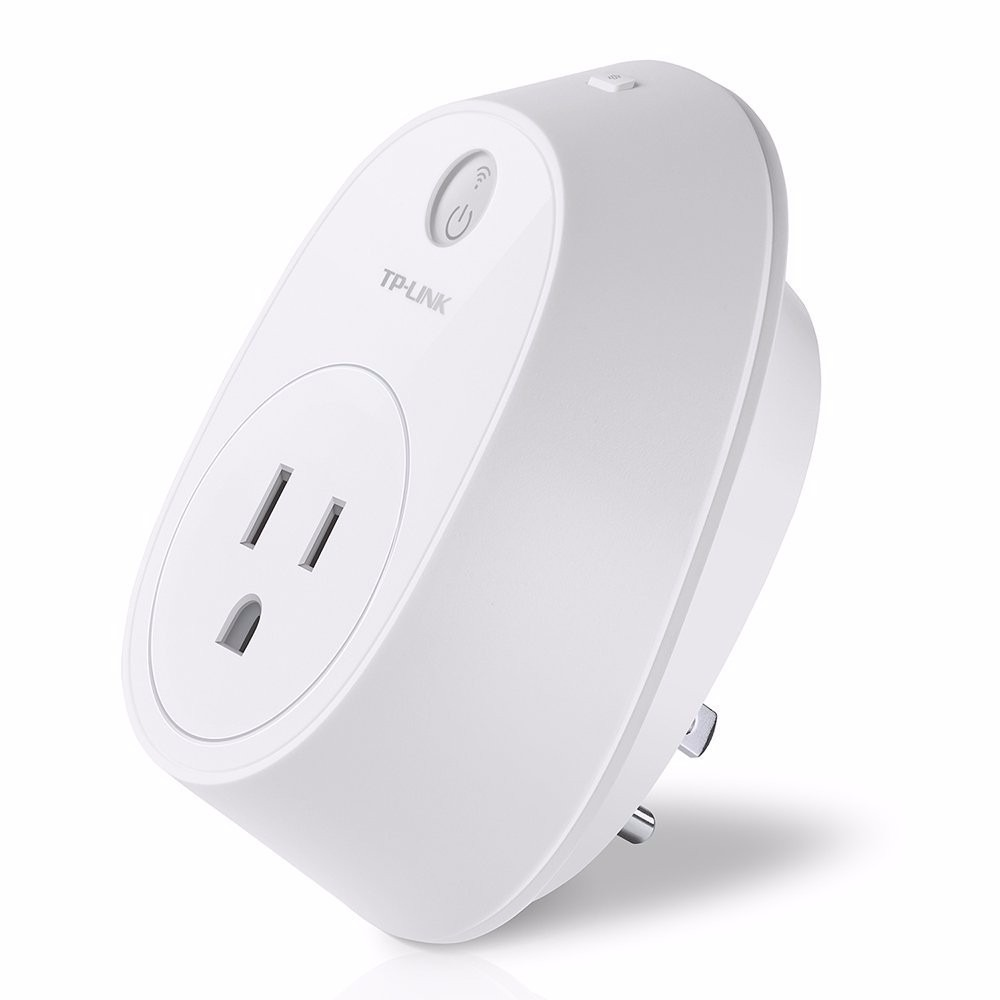
\includegraphics[width=6cm]{./Figures/1_2_TP-LINK-HS110.png}
	\caption{Smart Plug HS110 de la empresa TP-LINK}
	\label{fig:smartplug_tplink}
\end{figure}

\section{Objetivos}




%----------------------------------------------------------------------------------------






